% Permission is granted to copy, distribute and/or modify this document
% under the terms of the GNU Free Documentation License, Version 1.3
% or any later version published by the Free Software Foundation;
% with no Invariant Sections, no Front-Cover Texts, and no Back-Cover Texts.
% A copy of the license is included in the section entitled "GNU
% Free Documentation License".
%
% Written (C) 2012 Chiyuan Zhang

\chapter{Multiclass learning}

In this chapter we describe multiclass learning algorithms available in the 
\shogun{} toolbox.  Multiclass learning refers to the problem with the output 
space $\mathcal{Y}=\{1,\ldots,K\}$\footnote{Note while we describe the class 
	numbers as from $1$ to $K$, the multiclass machines in \shogun{} expect 
	the examples to be labeled with $0,\ldots,K-1$.}, where $K>2$.  Most of 
real world machine learning classification problems are naturally multiclass.   
Typical examples include document categorization, image classification, 
hand-written digit recognition, etc.  

Generally, no assumption of any specific structure for the set $\mathcal{Y}$
are made in multiclass learning.  When priori knowledge are available for a
rich structure of $\mathcal{Y}$, \emph{structured-output learning} algorithms
are usually used instead.

Many algorithms, like K-Nearest Neighbors and Naive Bayes, handle both 
multiclass problems and binary problems naturally (and in an uniform way). 
Those are described in section~\ref{sec:multiclass-natural}. 
Section~\ref{sec:multiclass-reduction} describes reduction from multiclass 
problems into binary problems. Tree-styled classifiers are described in 
section~\ref{sec:multiclass-tree}.

Several standard datasets are used by examples in this chapter. We summarize
them in Table~\ref{tab:multiclass-dataset}. All of those datasets can be found
in \url{http://mldata.org}.

\begin{table}[t]\centering
	\begin{tabular}{ccccc}
		\toprule
		Name & \# Classes & \# Samples & \# Attributes & Remarks \\
		\midrule
		USPS & 10         & 9298       & 256           & Hand-written Digits \\
		\bottomrule
	\end{tabular}
	\caption{Standard datasets for multiclass learning used in examples.}
	\label{tab:multiclass-dataset}
\end{table}

\section{Natural Multiclass Algorithms}
\label{sec:multiclass-natural}

\subsection{K-Nearest Neighbors}
\emph{K-Nearest Neighbors} (KNN) is a very simple and effective algorithm. The 
learning step actually does nothing but memorizing all the training points and 
the associated labels. The prediction is carried out by finding the $K$ 
nearest neighbors of the query point, and then voting.  Here $K$ is a 
hyper-parameter for the algorithm. Smaller $K$ gives the model low bias but 
high variance; while larger $K$ gives low variance but high bias.

KNN has attracted focus from both industrial and academia ever since its
conception. It is easy to implement, and can handle almost arbitrarily complex
problem by adjusting one single parameter $K$. Besides, it also has many nice
theoretical properties \citep{ProbTheoryofPR}.

In \shogun, you can use \shogunclass{CKNN} to perform KNN learning. To
construct a KNN machine, you must choose the hyper-parameter $K$ and a distance
function. Usually, we simply use the \shogunclass{CEuclideanDistance}, but in
general, any subclass of \shogunclass{CDistance} can be used. For
demonstration, we select a random subset of 1000 samples from USPS, and run
2-fold cross validation of KNN on it with varying $K$. The accuracy is shown in
Fig.~\ref{fig:mc-knn-acc}.

In \shogun{}, you can also use \emph{Cover Tree} \citep{CoverTree} to speed up
the nearest neighbor searching process in KNN. Just call \Verb|set_use_covertree| on
the KNN machine to enable or disable this feature. The prediction time
comparison for this experiment with and without Cover Tree are shown in
Fig.~\ref{fig:mc-knn-time}.

\begin{figure}\centering
	\begin{subfigure}{.48\textwidth}
		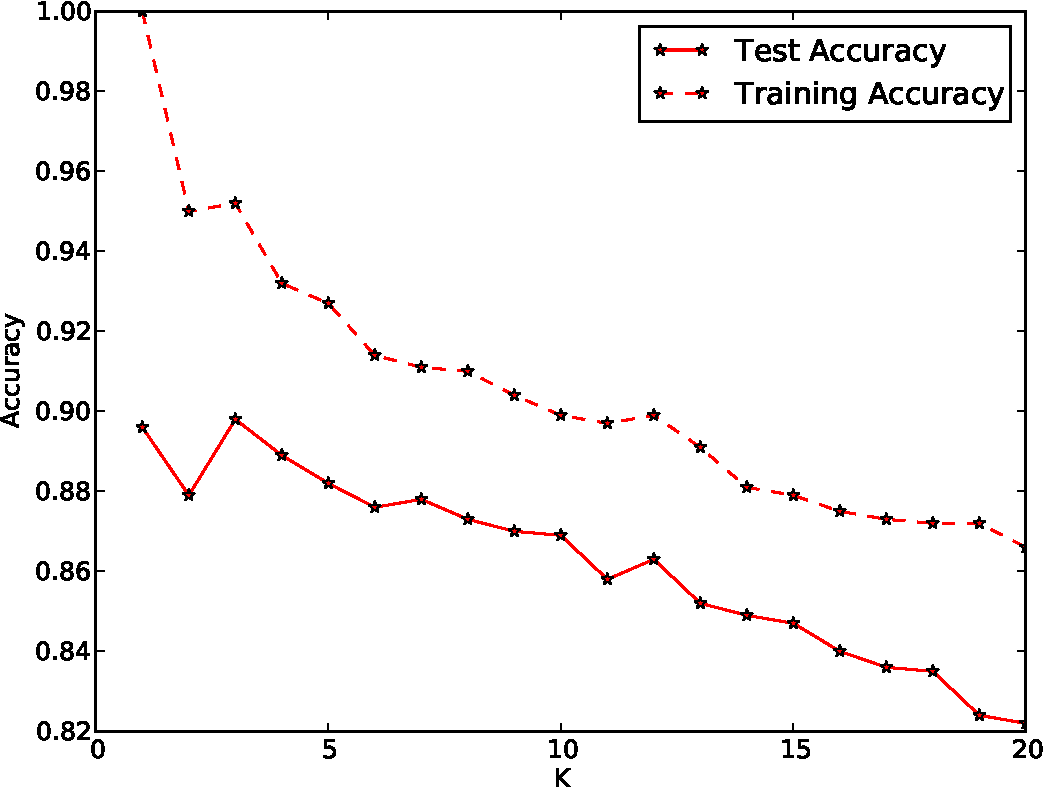
\includegraphics{fig/multiclass/knn-accuracy}
		\caption{KNN classification accuracy on USPS.}
		\label{fig:mc-knn-acc}
	\end{subfigure}
	~
	\begin{subfigure}{.48\textwidth}
		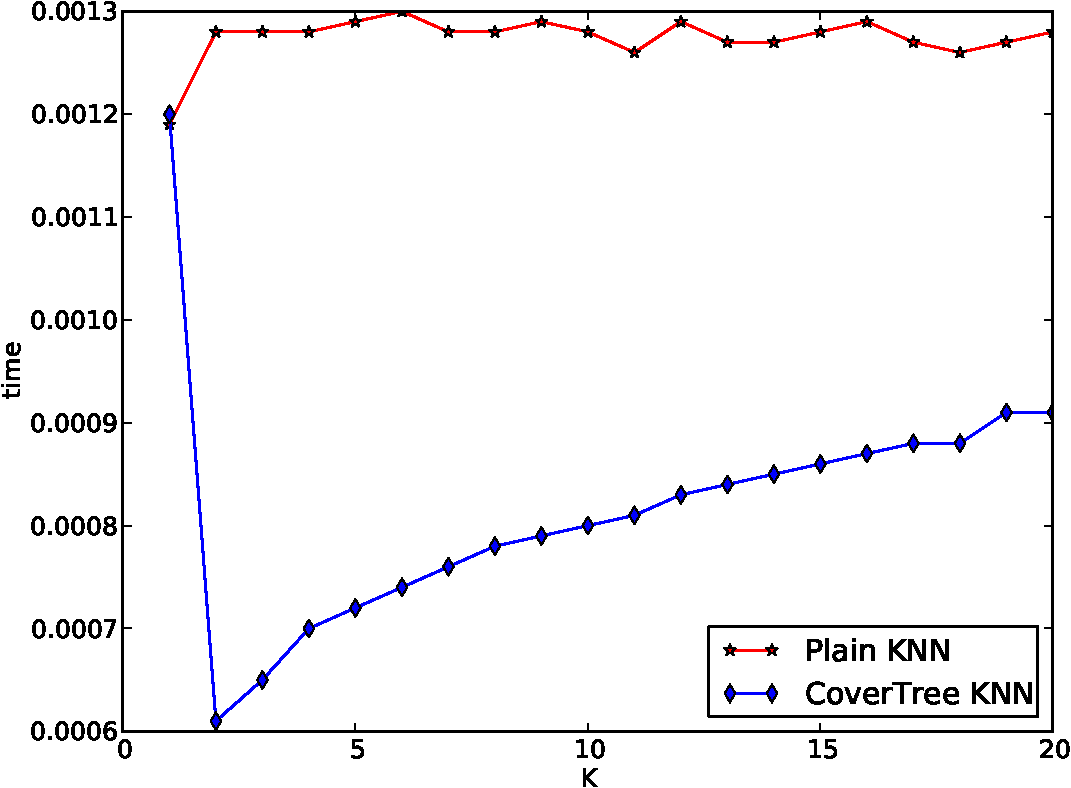
\includegraphics{fig/multiclass/knn-time}
		\caption{Prediction time (per example) with and without CoverTree.}
		\label{fig:mc-knn-time}
	\end{subfigure}
	\caption{KNN classification on a random subset (1000 samples) of USPS.}
\end{figure}

Although simple and elegant, KNN is generally very resource costly. Because all
the training samples are to be memorized literally, the memory cost of KNN
``learning'' becomes prohibitive when the dataset is huge. Even though the
memory is big enough to hold all the data, the prediction will be slow, since
the distances between the query point and all the training points need to be
computed and ranked. The situation becomes worse if in addition the data
samples are all very high-dimensional.

\subsection{Naive Bayes}
\emph{Naive Bayes} is a simple and fast algorithm for multiclass learning.
Formally, it predict the class by computing the posterior probability of each
class $k$ after observing the input $x$:

\[
	P\left( Y=k | X = x \right) = \frac{P(X=x|Y=k)P(Y=k)}{P(X=x)}
\]

The prediction is then made by

\[
	y = \argmax_{k\in\{1,\ldots,K\}} P(Y=k|X=x)
\]

Since $P(X=x)$ is a constant factor for all $P(Y=k|X=x)$, $k=1,\ldots,K$, there
is no need to compute it.

In \shogun{}, \shogunclass{CGaussianNaiveBayes} implements the Naive Bayes
algorithm. It is prefixed with ``Gaussian'' because the probability model for
$P(X=x|Y=k)$ for each $k$ is taken to be a multi-variate Gaussian distribution.
Furthermore, each dimension of the feature vector $X$ is assumed to be
independent. The ``Naive'' independence assumption enables us the learn the
model by estimating the parameters for each feature dimension independently,
thus the whole learning algorithm runs very quickly. And this is also the 
reason for its name. However, this assumption can be very restrictive. In
Fig.~\ref{fig:mc-gnb-fail}, we show a simple 2D example. There are 3 linearly
separable classes. The scattered points are training samples with colors
indicating their labels. The filled area indicate the hypothesis learned by
the \shogunclass{CGaussianNaiveBayes}. The training samples are actually
generated from three Gaussian distributions. But since the covariance for those
Gaussian distributions are not diagonal (i.e. there are ``rotations''), the GNB
algorithm cannot handle them properly.

\begin{figure}
    \centering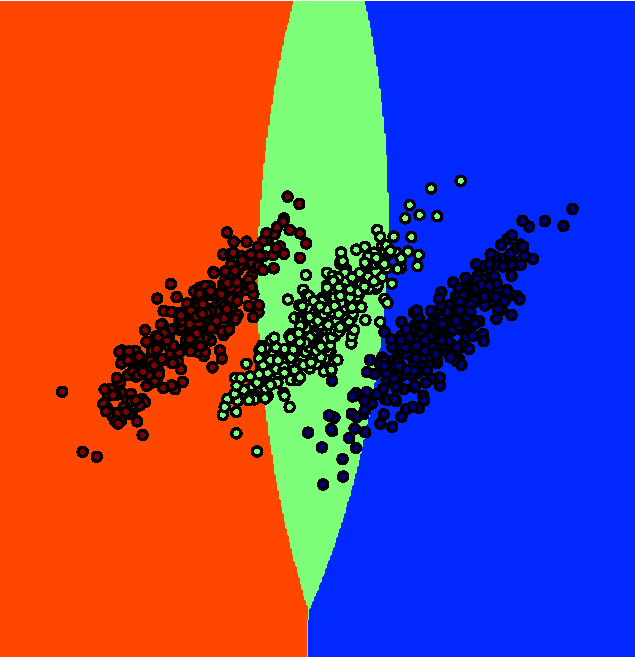
\includegraphics{fig/multiclass/gnb-fail-case}
    \caption{Gaussian Naive Bayes fails to learn on a simple 2D example with 3
    linearly separable classes.}
    \label{fig:mc-gnb-fail}
\end{figure}

Although the independent assumption is usually considered to be too optimistic 
in reality, Naive Bayes sometimes works very well in some applications. For 
example, in email spam filtering, Naive Bayes\footnote{More specifically, the 
    discrete Naive Bayes is generally used in this scenario. The main 
    difference with Gaussian Naive Bayes is that a tabular instead of a 
    parametric Gaussian distribution is used to describe the likelihood 
    $P(X=x|K=k)$.} is a very popular and widely used method.

This algorithm is closely related to the \emph{Gaussian Mixture Model} (GMM) learning
algorithm. However, while GMM is an unsupervised learning algorithm, Gaussian
Naive Bayes is supervised learning. It uses the training labels to directly
estimate the Gaussian parameters for each class, thus avoids the iterative
\emph{Expectation Maximization} procedures in GMM.

The merit of GNB is that both training and predicting are very fast, and it has
no hyper-parameters.

\subsection{Logistic Regression}

Although named logistic \emph{regression}, it is actually a classification
algorithm. Similar to \emph{Naive Bayes}, logistic regression computes the
posterior $P(Y=k|X=x)$ and makes prediction by

\[
    y = \argmax_{k\in\{1,\ldots,K\}} P(Y=k|X=x)
\]

However, Naive Bayes is a \emph{generative model}, in which the distribution of
the input variable $X$ is also modeled (by a Gaussian distribution in this
case). But logistic regression is a \emph{discriminative model}, which doesn't
care about the distribution of $X$, and models the posterior directly.
Actually, the two algorithms are a \emph{generative-discriminative pair}
\citep{DBLP:conf/nips/NgJW01}.

To be specific, logistic regression uses \emph{linear} functions in $X$ to model the
posterior probabilities:

\begin{eqnarray}
    \log\frac{P(Y=1|X=x)}{P(Y=K|X=x)} &=& \beta_{10} + \beta_1^Tx \\
    \log\frac{P(Y=2|X=x)}{P(Y=K|X=x)} &=& \beta_{20} + \beta_2^Tx \\
    &\vdots& \nonumber\\
    \log\frac{P(Y=K-1|X=x)}{P(Y=K|X=x)} &=& \beta_{(K-1)0} + \beta_{K-1}^Tx
\end{eqnarray}

The training of a logistic regression model is carried out via \emph{maximum
    likelihood estimation} of the parameters
$\boldsymbol\beta = \{\beta_{10},\beta_1^T,\ldots,\beta_{(K-1)0},\beta_{K-1}^T\}$. There is no
closed form solution for the estimated parameters.

There is not independent implementation of logistic regression in \shogun{}, 
but the \shogunclass{CLibLinear} becomes a logistic regression model when
constructed with the argument \Verb|L2R_LR|. This model also include a
regularization term of the $\ell_2$-norm of $\boldsymbol\beta$. If sparsity in
$\boldsymbol\beta$ is needed, one can also use \Verb|L1R_LR|, which replaces
the $\ell_2$-norm regularizer with a $\ell_1$-norm regularizer.

Unfortunately, the logistic regression in \shogun{} does not support multiclass
problem yet.

\section{Reduction to Binary Problems}
\label{sec:multiclass-reduction}

Since binary classification problems are one of the most thoroughly studied
problems in machine learning, it is very appealing to consider reducing
multiclass problems to binary ones. Then many advanced learning and
optimization techniques as well as generalization bound analysis for binary
classification can be utilized.

In \shogun{}, the strategies of reducing a multiclass problem to binary
classification problems are described by an instance of
\shogunclass{CMulticlassStrategy}. A multiclass strategy describes
\begin{enumerate}
\item How to train the multiclass machine as a number of binary machines?
	\begin{itemize}
		\item How many binary machines are needed?
		\item For each binary machine, what subset of the training samples are
			used, and how are they colored\footnote{In multiclass problems, we
				use \emph{coloring} to refer partitioning the classes into two
				groups: $+1$ and $-1$, or black and white, or any other meaningful
				names.}?
	\end{itemize}
\item How to combine the prediction results of binary machines into the final
	multiclass prediction?
\end{enumerate}

The user can derive from the virtual class \shogunclass{CMulticlassStrategy} to
implement a customized multiclass strategy. But usually the built-in strategies
are enough for general problems. We will describe the built-in \emph{One-vs-Rest},
\emph{One-vs-One} and \emph{Error-Correcting Output Codes} strategies in the
following subsections.

The basic routine to use a multiclass machine with reduction to binary problems
in shogun is to create a generic multiclass machine and then assign a particular
multiclass strategy and a base binary machine.

\subsection{One-vs-Rest and One-vs-One}

The \emph{One-vs-Rest} strategy is implemented in
\shogunclass{CMulticlassOneVsRestStrategy}. As indicated by the name, this
strategy reduce a $K$-class problem to $K$ binary sub-problems. For the $k$-th
problem, where $k\in\{1,\ldots,K\}$, the samples from class $k$ are colored as
$+1$, and the samples from other classes are colored as $-1$. The multiclass
prediction is given as

\[
	f(x) = \argmax_{k\in\{1,\ldots,K\}} f_k(x)
\]
where $f_k(x)$ is the prediction of the $k$-th binary machines.

The One-vs-Rest strategy is easy to implement yet produces the good performance
in many cases. One interesting paper \citep{OneVsRestDefense} shows that the
One-vs-Rest strategy can be

\begin{quote}
	\emph{as accurate as any other approach, assuming that the underlying binary
classifiers are well-tuned regularized classifiers such as support vector
machines.}
\end{quote}

Implemented in \shogunclass{CMulticlassOneVsOneStrategy}, the 
\emph{One-vs-One} strategy \citep{OneVsOne} is another simple and intuitive 
strategy: it basically produces one binary problem for each pair of classes.  
So there will be $\binom{K}{2}$ binary problems. At prediction time, the 
output of every binary classifiers are collected to do voting for the $K$ 
classes. The class with the highest vote becomes the final prediction.

Compared with the One-vs-Rest strategy, the One-vs-One strategy is usually more
costly to train and evaluate because more binary machines are used.

In the following, we demonstrate how to use \shogun{}'s One-vs-Rest and 
One-vs-One multiclass learning strategy on the USPS dataset.  For 
demonstration, we randomly 200 samples from each class for training and 200 
samples from each class for testing.
\todo[inline]{How to organize and reference example code for tutorial?}

\begin{table}\centering
	\begin{tabular}{cccc}
	\toprule
	Strategy & Training Time & Test Time & Accuracy \\
	\midrule
	One-vs-Rest & 1.72       & 2.25      & 92.05\%  \\
	One-vs-One  & 2.14       & 4.45      & 93.75\%  \\
	\bottomrule
	\end{tabular}
	\caption{Comparison of One-vs-Rest and One-vs-One multiclass reduction
		strategy on the USPS dataset.}
	\label{tab:ovr-vs-ovo}
\end{table}

The \shogunclass{CLibLinear} is used as the base binary classifier in a
\shogunclass{CLinearMulticlassMachine}, with One-vs-Rest and One-vs-One
strategies. The running time and performance is reported in
Table~\ref{tab:ovr-vs-ovo}.

\subsection{Error-Correcting Output Codes}

\emph{Error-Correcting Output Codes} (ECOC) \citep{ECOC95,ECOCUnify} is a
generalization of the One-vs-Rest and One-vs-One strategies. For example, we
can represent the One-vs-Rest strategy with the following $K\times K$ coding 
matrix, or a codebook:

\[
    \begin{bmatrix}
    +1 & -1 & -1 & \ldots & -1 & -1 \\
    -1 & +1 & -1 & \ldots & -1 & -1\\
    -1 & -1 & +1 & \ldots & -1 & -1\\
    \vdots & \vdots & \vdots & \ddots & \vdots & \vdots \\
    -1 & -1 & -1 & \ldots & +1 & -1 \\
    -1 & -1 & -1 & \ldots & -1 & +1
    \end{bmatrix}
\]

Denote the codebook by $B$, there is one column of the codebook associated with
each of the $K$ classes. For example, the code for class $1$ is
$[+1,-1,-1,\ldots,-1]$. Each row of the codebook corresponds to a binary
coloring of all the $K$ classes. For example, in the first row, the class $1$
is colored as $+1$, while the rest of the classes are all colored as $-1$.
Associated with each row, there is a binary classifier trained according to the
coloring. For example, the binary classifier associated with the first row is
trained by treating all the examples of class $1$ as positive examples, and all
the examples of the rest of the classes as negative examples.

In this special case, there are $K$ rows in the codebook. The number of rows in
the codebook is usually called the \emph{code length}. As we can see, this
codebook exactly describes how the One-vs-Rest strategy trains the binary
sub-machines.

A further generalization is to allow $0$-values in the codebook. A $0$ for a
class $k$ in a row means we ignore (the examples of) class $k$ when training
the binary classifiers associated with this row. With this generalization, we
can also easily describes the One-vs-One strategy with a $\binom{K}{2}\times K$
codebook:

\[
\begin{bmatrix}
+1     & -1     & 0      & \ldots & 0      & 0 \\
+1     & 0      & -1     & \ldots & 0      & 0 \\
\vdots & \vdots & \vdots & \ddots & \vdots & 0 \\
+1     & 0      & 0      & \ldots & -1     & 0 \\
0      & +1     & -1     & \ldots & 0      & 0 \\
\vdots & \vdots & \vdots &        & \vdots & 0 \\
0      & 0      & 0      & \ldots & +1     & -1
\end{bmatrix}
\]

Here each of the $\binom{K}{2}$ rows describes a binary classifier trained with
a pair of classes. The resultant binary classifiers will be identical as those
described by a One-vs-One strategy.

Since $0$ is allowed in the codebook to ignore some classes, this kind of
codebooks are usually called \emph{sparse codebook}s, while the codebooks with
only $+1$ and $-1$ are usually called \emph{dense codebook}.

In general case, we can specify any code length and fill the codebook
arbitrarily. However, some rules should be followed:

\begin{enumerate}
    \item Each row must describe a \emph{valid} binary coloring. In other
        words, both $+1$ and $-1$ should appear at least once in each row. Or
        else a binary classifier cannot be obtained for this row.
    \item It is good to avoid duplicated rows. There is generally no harm to
        have duplicated rows, but the resultant binary classifiers are
        completely identical provided the training algorithm for the binary
        classifiers are deterministic. So this can be a waste of computational
        resource.
    \item Negative rows are also duplicated. Simply inversing the sign of a code
        row does not produce a ``new'' code row. Because the resultant binary
        classifier will simply be the negative classifier associated with the
        original row.
\end{enumerate}

Though you can certainly generate your own codebook, it is usually easier to
use the \shogun{} built-in procedures to generate codebook automatically. There
are various codebook generators (called \emph{encoders}) in \shogun{}. However,
before describing those encoders in details, let us notice that a codebook 
only describes how the sub-machines are trained. But we still need a
way to specify how the binary classification results of the sub-machines can be
combined to get a multiclass classification result.

Describe the name ECOC here, and describe the \shogun{} ECOC encoding/decoding
pairs.

\section{Tree-style Algorithms}
\label{sec:multiclass-tree}
